%%% LaTeX Template: Article/Thesis/etc. with colored headings and special fonts
%%%
%%% Source: http://www.howtotex.com/
%%% Feel free to distribute this template, but please keep to referal to http://www.howtotex.com/ here.
%%% February 2011
%%%
%%% Modified January 2016 by CDM

%%%  Preamble
\documentclass[11pt,letterpaper]{article}
\usepackage[margin=1.0in]{geometry}
\usepackage[T1]{fontenc}
\usepackage[bitstream-charter]{mathdesign}
\usepackage[latin1]{inputenc}					
\usepackage{amsmath}						
\usepackage{xcolor}
\usepackage{cite}
\usepackage{hyphenat}
\usepackage{graphicx}
\usepackage{float}
\usepackage{subfigure}
\usepackage{sectsty}
\usepackage[compact]{titlesec} 
\usepackage[tablegrid]{vhistory}
\usepackage{pbox}
\allsectionsfont{\color{accentcolor}\scshape\selectfont}

%%% Definitions
\definecolor{accentcolor}{rgb}{0.0,0.0,0.5} 
\newcommand{\teamname}{Team Telepresence}
\newcommand{\productname}{Rift Telepresence}
\newcommand{\coursename}{CSE 4317: Senior Design II}
\newcommand{\semester}{Spring 2017}
\newcommand{\docname}{Architectural Design Specification}
\newcommand{\department}{Department of Computer Science \& Engineering}
\newcommand{\university}{The University of Texas at Arlington}
\newcommand{\authors}{Cameron Adams \\ John Green \\ Andy Le \\ Clement Olayiwola \\ Ty Simmel}

%%% Headers and footers
\usepackage{fancyhdr}
	\pagestyle{fancy}						% Enabling the custom headers/footers
\usepackage{lastpage}	
	% Header (empty)
	\lhead{}
	\chead{}
	\rhead{}
	% Footer
	\lfoot{\footnotesize \teamname \ - \semester}
	\cfoot{}
	\rfoot{\footnotesize page \thepage\ of \pageref{LastPage}}	% "Page 1 of 2"
	\renewcommand{\headrulewidth}{0.0pt}
	\renewcommand{\footrulewidth}{0.4pt}

%%% Change the abstract environment
\usepackage[runin]{abstract}			% runin option for a run-in title
%\setlength\absleftindent{30pt}			% left margin
%\setlength\absrightindent{30pt}		% right margin
\abslabeldelim{\quad}	
\setlength{\abstitleskip}{-10pt}
\renewcommand{\abstractname}{}
\renewcommand{\abstracttextfont}{\color{accentcolor} \small \slshape}	% slanted text

%%% Start of the document
\begin{document}

%%% Cover sheet
{\centering \huge \color{accentcolor} \sc \textbf{\department \\ \university} \par}
\vspace{1 in}
{\centering \huge \color{accentcolor} \sc \textbf{\docname \\ \coursename \\ \semester} \par}
\vspace{0.5 in}
\begin{figure}[h!]
	\centering
   	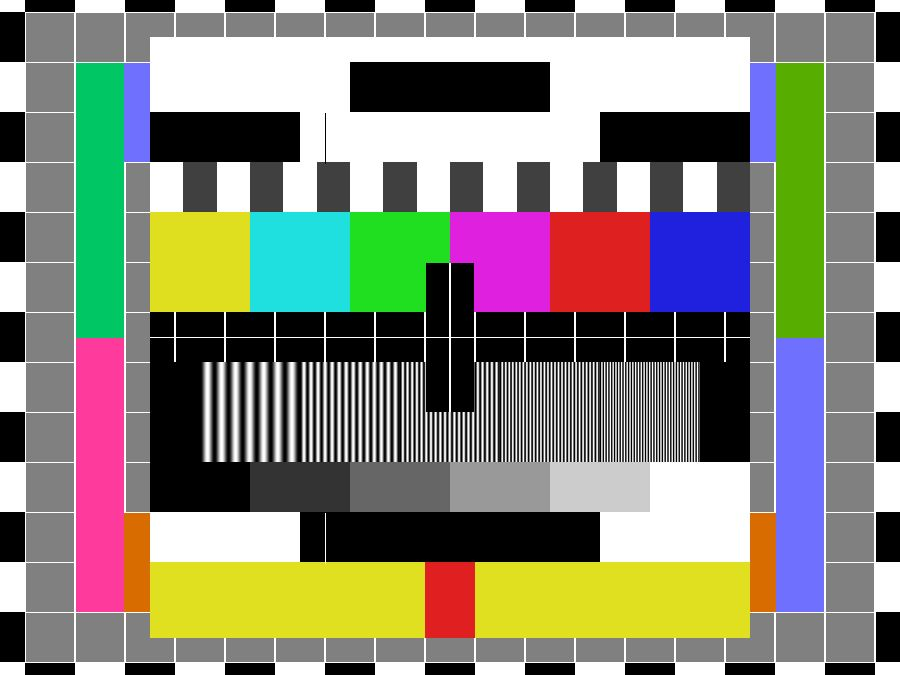
\includegraphics[width=0.60\textwidth]{images/test_image}
\end{figure}
\vspace{0.5 in}
{\centering \huge \color{accentcolor} \sc \textbf{\teamname \\ \productname} \par}
\vspace{0.5 in}
{\centering \large \sc \textbf{\authors} \par}
\newpage


%\vspace{1 in}
%\centerline{January 13th, 2012}
%\newpage

%%% Revision History
\begin{versionhistory}
  	\vhEntry{0.1}{10.25.2016}{CA|JG|AL|CO|TS}{Document creation}
  	\vhEntry{0.2}{12.15.2016}{CA|JG|AL|CO|TS}{Removed Mobile Platform Layer}
  	\vhEntry{0.3}{04.19.2017}{CA|JG|AL|CO|TS}{Update document}
\end{versionhistory}
\newpage

%%% Table of contents
\setcounter{tocdepth}{2}
\tableofcontents
\newpage

%%% List of figures and tables (optional)
\listoffigures
\listoftables
\newpage

%%% Document sections
\section{Introduction}
The project will be a custom stereoscopic camera mounted on a gimbal with 3D movement capabilites (pitch, yaw, roll). The movement of the cameras will be one-to-one with the movement of a virtual reality headset on the user. Minimal computation will be used onboard the actual unit. The majority of processing will be accomplished by the computer running the virtual reality headset. Camera focal points will be preset and calibrated to predetermine the focal distance. Initial versions of the system will use a wire tether for data transfer between the camera unit and processing unit.
\newpage
\section{System Overview}
The Camera System handles three primary tasks. The motor controller board receives signals from the Processing System. The control board then orients the gimbal to the angles specified by the signals. For the final task, the cameras capture stereo video and pass the video to the Processing System. The Processing System serves as an intermediary between the Camera System and Virtual Reality System. The two functionalities are processing the video and translating the head tracking data. The final system is the Virtual Reality System. This system is responsible for the stereo display of the video and the capture of the raw head tracking data.

\begin{figure}[h!]
	\centering
 	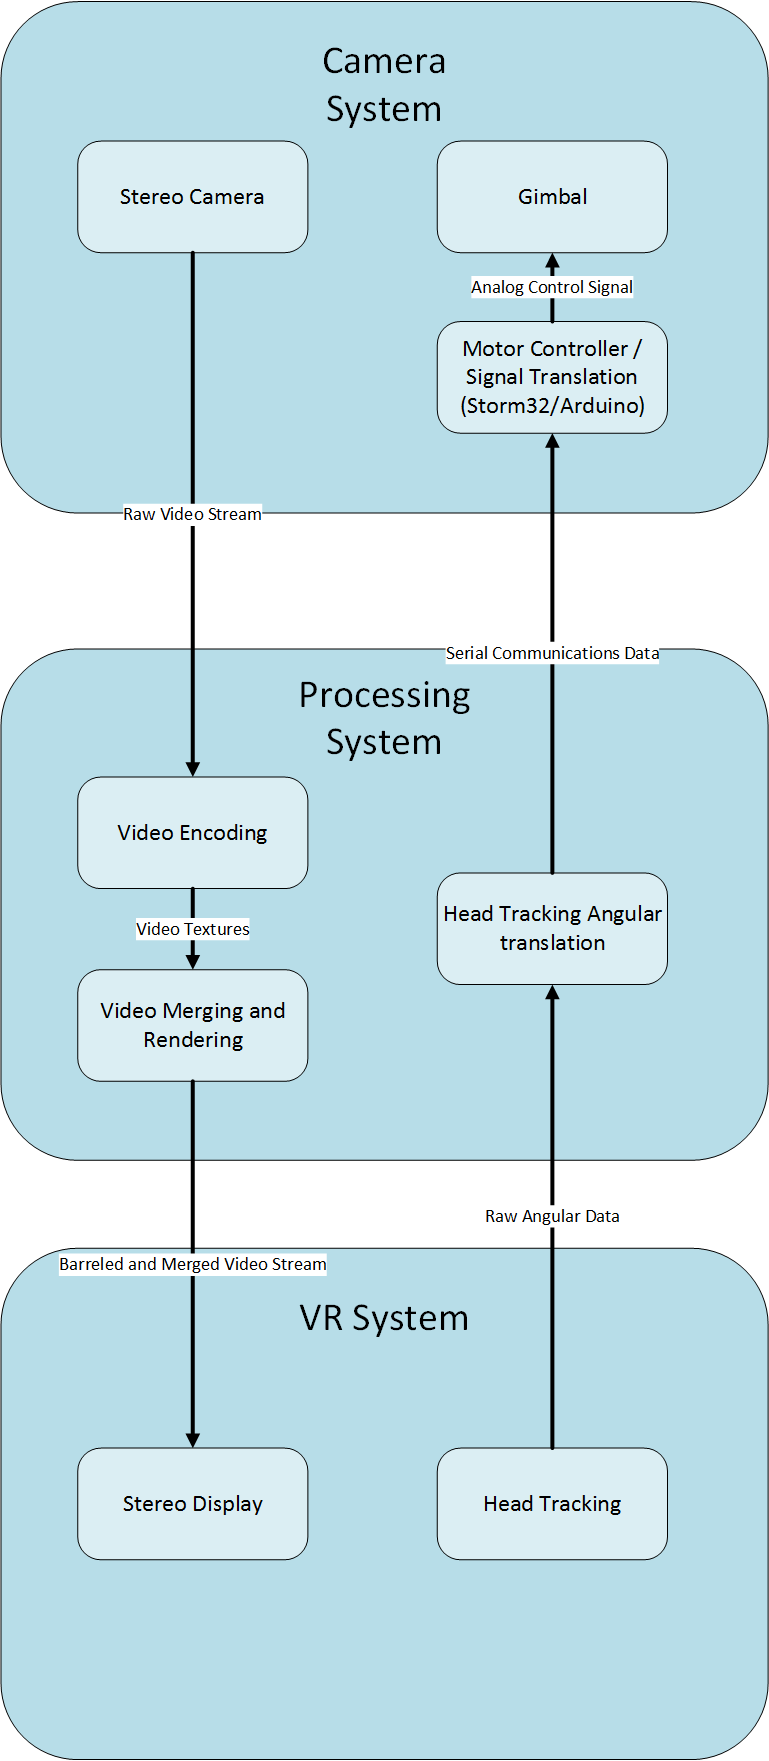
\includegraphics[width=0.27\textwidth]{images/Overview}
 \caption{System architecture}
\end{figure}

\newpage
\section{Subsystem Definitions \& Data Flow}
\begin{figure}[h!]
	\centering
 	\includegraphics[width=0.52\textwidth]{images/overview}
	\caption{Data flow diagram of system}
\end{figure}

\newpage
\section{Camera System Layer Subsystems}
The Camera System Layer contains a camera subsystem, gimbal subsystem, and gimbal controller subsystem. These subsystems send raw video streams to the Processing System Layer and receive head tracking angles from it.

\begin{figure}[h!]
	\centering
 	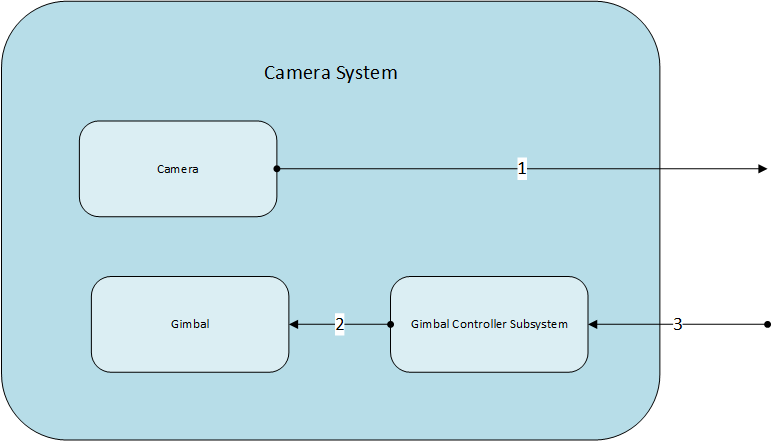
\includegraphics[width=0.75\textwidth]{images/camerasubsystem}
 \caption{Camera System Layer Subsystem Description Diagram}
\end{figure}

\subsection{Camera Subsystem}
The camera subsystem will send the raw video streams directly to the Processing System to be processed.

\subsubsection{Assumptions}
This subsystem is assumed to be handled by the firmware already built into the cameras.

\subsubsection{Responsibilities}
This subsystem is responsible for giving video input to the system that will eventually end up in the virtual reality headset the user is wearing.

\subsubsection{Subsystem Interfaces}
This subsystem will have a one-way interface which is with the Processing System's video input subsystem. Through this interface, the raw video will be streamed and processed.

\begin {table}[H]
\caption {Camera Subsystem interfaces} 
\begin{center}
    \begin{tabular}{ | p{1cm} | p{6cm} | p{3cm} | p{3cm} |}
    \hline
    ID & Description & Inputs & Outputs \\ \hline
    \#1 & Processing System - Video Input Subsystem & \pbox{3cm}{N/A} & \pbox{3cm}{Raw video footage}  \\ \hline
    \end{tabular}
\end{center}
\end{table}

\subsection{Gimbal Subsystem}
This subsystem communicates with the gimbal controller subsystem to move each gimbal motor to their position.

\subsubsection{Assumptions}
Head tracking angles are read in a certain order from the translations of angles from the gimbal controller subsystem's serial communication.

\subsubsection{Responsibilities}
This subsystem is responsible for the movement of the gimbals by reading and moving into the positions given by the gimbal controller subsystem's head tracking angles.

\subsubsection{Subsystem Interfaces}
This subsystem will have a one-way interface. Head tracking angles are received from the gimbal controller subsystem.

\begin {table}[H]
\caption {Gimbal Subsystem interfaces} 
\begin{center}
    \begin{tabular}{ | p{1cm} | p{6cm} | p{3cm} | p{3cm} |}
    \hline
    ID & Description & Inputs & Outputs \\ \hline
    \#2 & Gimbal Controller Subsystem & \pbox{3cm}{Translated head tracking angles} & \pbox{3cm}{N/A}  \\ \hline
    \end{tabular}
\end{center}
\end{table}

\subsection{Gimbal Controller Subsystem}
Head tracking data will be received and handled in this subsystem from the Processing System before sending the resulting data to the gimbal subsystem.

\subsubsection{Assumptions}
None

\subsubsection{Responsibilities}
This subsystem will receive the head tracking angles from the Processing System. It will then translate the angles to be sent to the gimbal subsystem.

\subsubsection{Subsystem Interfaces}
This subsystem will have two one-way interface. The Processing system will send the data to this subsystem which will then send it to the gimbal subsystem.

\begin {table}[H]
\caption {Gimbal Controller Subsystem interfaces} 
\begin{center}
    \begin{tabular}{ | p{1cm} | p{6cm} | p{3cm} | p{3cm} |}
    \hline
    ID & Description & Inputs & Outputs \\ \hline
    \#3 & Gimbal Subsystem & \pbox{3cm}{N/A} & \pbox{3cm}{Translated head tracking angles}  \\ \hline
     \#4 & Processing System -  Gimbal Controller Subsystem & \pbox{3cm}{Head tracking angles} & \pbox{3cm}{N/A}  \\ \hline
    \end{tabular}
\end{center}
\end{table}
\newpage
\section{Processing System Layer Subsystems}
This system contains the video input subsystem, the video output subsystem, and the gimbal controller subsystem. Each subsystem makes it possible for this system to communicate with the Camera System Layer and the Virtual Reality System Layer. Video data will be received from the Camera System Layer and transferred to the Virtual Reality System Layer, while angular data will be received from the Virtual Reality System Layer and sent to the Camera System Layer.

\begin{figure}[h!]
	\centering
 	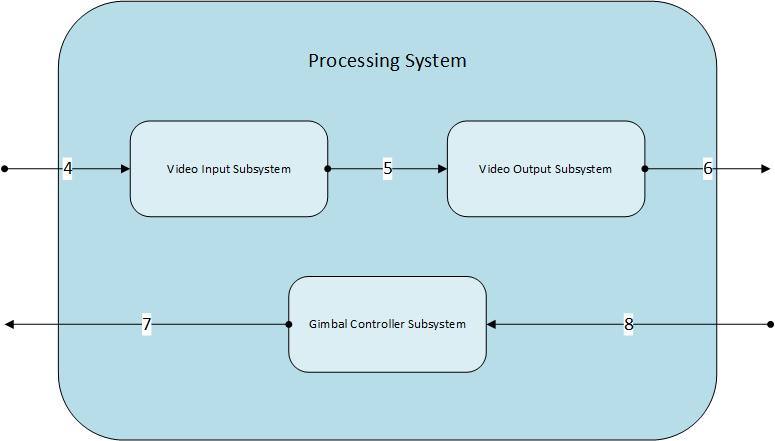
\includegraphics[width=0.75\textwidth]{images/processingsubsystem}
 \caption{Microcomputer System Layer Subsystem Description Diagram}
\end{figure}

\subsection{Video Input Subsystem}
This subsystem communicates with the camera subsystem in the Camera System Layer. Also, the video interface subsystem interacts with the video output subsystem in this system.

\subsubsection{Assumptions}
None

\subsubsection{Responsibilities}
This subsystem will receive raw video data sent from the Camera System Layer. The raw video data will then be processed and sent to the video output subsystem in this system.

\subsubsection{Subsystem Interfaces}

\begin {table}[H]
\caption {Video Input Subsystem interfaces} 
\begin{center}
    \begin{tabular}{ | p{1cm} | p{6cm} | p{3cm} | p{3cm} |}
    \hline
    ID & Description & Inputs & Outputs \\ \hline
    \#5 & Camera System - Camera Subsystem & \pbox{3cm}{Raw video data} & \pbox{3cm}{N/A}  \\ \hline
    \#6 & Video Output Subsystem & \pbox{3cm}{N/A} & \pbox{3cm}{Processed video data}  \\ \hline
    \end{tabular}
\end{center}
\end{table}

\subsection{Video Output Subsystem}
This subsystem interacts with the video input subsystem in this system, and it will be one of the means of communication between the Processing System Layer and the Virtual Reality System Layer.

\subsubsection{Assumptions}
None

\subsubsection{Responsibilities}
Processed video data is received from the video input subsystem in this system. With the video data, it will be transferred to the Virtual Reality System Layer to be displayed.

\subsubsection{Subsystem Interfaces}

\begin {table}[H]
\caption {Video Output Subsystem interfaces} 
\begin{center}
    \begin{tabular}{ | p{1cm} | p{6cm} | p{3cm} | p{3cm} |}
    \hline
    ID & Description & Inputs & Outputs \\ \hline
    \#7 & Video Input Subsystem & \pbox{3cm}{Processed video data} & \pbox{3cm}{N/A}  \\ \hline
    \#8 & Virtual Reality System - Stereo Display Subsystem & \pbox{3cm}{N/A} & \pbox{3cm}{Processed video data}  \\ \hline
    \end{tabular}
\end{center}
\end{table}

\subsection{Gimbal Controller Subsystem}
This subsystem interacts with the gimbal controller subsystem of the Camera System Layer and the head tracking subsystem of the Virtual Reality System Layer.

\subsubsection{Assumptions}
None

\subsubsection{Responsibilities}
This subsystem will take the raw angular data taken from the virtual reality headset of the Virtual Reality System Layer and send it to the gimbal controller subsystem of the Camera System Layer through serial communication.

\subsubsection{Subsystem Interfaces}

\begin {table}[H]
\caption {Gimbal Controller Subsystem interfaces} 
\begin{center}
    \begin{tabular}{ | p{1cm} | p{6cm} | p{3cm} | p{3cm} |}
    \hline
    ID & Description & Inputs & Outputs \\ \hline
    \#9 & Camera System - Gimbal Controller Subsystem & \pbox{3cm}{N/A} & \pbox{3cm}{Head tracking angles}  \\ \hline
    \#10 & Virtual Reality System - Stereo Display Subsystem & \pbox{3cm}{Raw head tracking angles} & \pbox{3cm}{N/A}  \\ \hline
    \end{tabular}
\end{center}
\end{table}
\newpage
\section{Virtual Reality System Layer Subsystems}
The Virtual Reality System Layer is focused on delivering real-time video and tracking of the head movement on the virtual reality headset. This system contains the stereo display subsystem and the head tracking subsystem. Both of the subsystems make it possible to communicate with the Processing System Layer.

\begin{figure}[h!]
	\centering
 	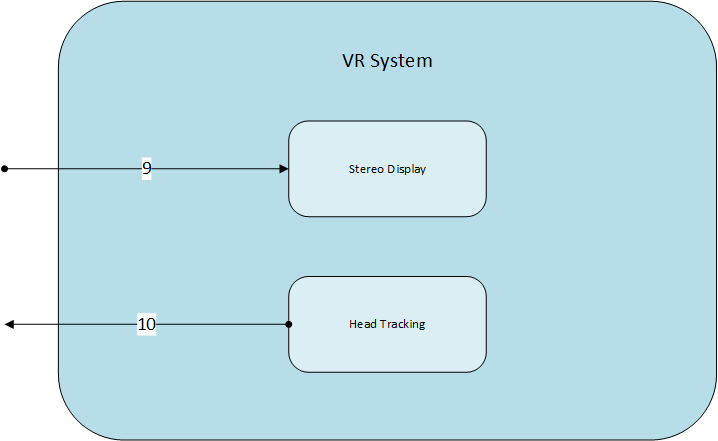
\includegraphics[width=0.75\textwidth]{images/vrsubsystem}
 \caption{Virtual Reality System Layer Subsystem Description Diagram}
\end{figure}

\subsection{Stereo Display Subsystem}
This subsystem interacts with the video output subsystem of the Processing System Layer by receiving the processed video data.

\subsubsection{Assumptions}
None

\subsubsection{Responsibilities}
The processed video data received from the Processing System Layer will be displayed through the user's virtual reality headset.

\subsubsection{Subsystem Interfaces}

\begin {table}[H]
\caption {Stereo Display Subsystem interfaces} 
\begin{center}
    \begin{tabular}{ | p{1cm} | p{6cm} | p{3cm} | p{3cm} |}
    \hline ID & Description & Inputs & Outputs \\ \hline
    \#11 & Processing System - Video Output Subsystem & \pbox{3cm}{Processed video data} & \pbox{3cm}{N/A}  \\ \hline
    \end{tabular}
\end{center}
\end{table}

\subsection{Head Tracking Subsystem}
This subsystem interacts with the gimbal controller subsystem of the Processing System Layer by sending head tracking data.

\subsubsection{Assumptions}
The accelerometer signals can be extracted from the headset. The accelerometer signals extracted from the headset can be decoded into standard PWM signals to control motor movement.

\subsubsection{Responsibilities}
Head tracking angles are taken from the user's virtual reality headset. The raw angular data will be sent to the gimbal controller subsystem of the Processing System Layer.

\subsubsection{Subsystem Interfaces}

\begin {table}[H]
\caption {Head Tracking Subsystem interfaces} 
\begin{center}
    \begin{tabular}{ | p{1cm} | p{6cm} | p{3cm} | p{3cm} |}
    \hline ID & Description & Inputs & Outputs \\ \hline
    \#12 & Processing System - Gimbal Controller Subsystem & \pbox{3cm}{N/A} & \pbox{3cm}{Raw head tracking angles}  \\ \hline
    \end{tabular}
\end{center}
\end{table}
\newpage

%%% References
\bibliographystyle{plain}
\bibliographystyle{reference/IEEEtran_custom}
\bibliography{reference/refs}{}

\end{document}